\section{The Lorenz System}

\begin{frame}{From Weather to Chaos}
  \begin{itemize}
    \item In the early 1960s, meteorologist \textbf{Edward Lorenz} was running a simple computer simulation of atmospheric convection.
    \item He restarted a run from the middle, rounding an intermediate value from $0.506127$ to $0.506$.
    \item The resulting trajectory diverged \textbf{completely} from the original.
    \item This accidental discovery became one of the founding stories of chaos theory.
    \item Lorenz later asked: \textit{``Does the flap of a butterfly's wings in Brazil set off a tornado in Texas?''}
  \end{itemize}
\end{frame}

\begin{frame}{The Lorenz Equations}
  The Lorenz system is a simplified model of convection rolls in a heated fluid:

  \begin{align*}
    \frac{dx}{dt} &= \sigma (y - x) \\[6pt]
    \frac{dy}{dt} &= \rho\, x - y - x\,z \\[6pt]
    \frac{dz}{dt} &= x\,y - b\,z
  \end{align*}

  \vfill

  \begin{tabular}{ll}
    $\sigma$ & Prandtl number (ratio of viscosity to thermal diffusivity) \\
    $\rho$   & Rayleigh number (driving force of convection) \\
    $b$      & geometric factor of the convection cell
  \end{tabular}

  \vfill
  Classical chaotic parameters: $\sigma = 10$, $\rho = 28$, $b = 8/3$.
\end{frame}

\begin{frame}{The Strange Attractor}
  \begin{columns}
    \column{0.55\textwidth}
    \begin{center}
      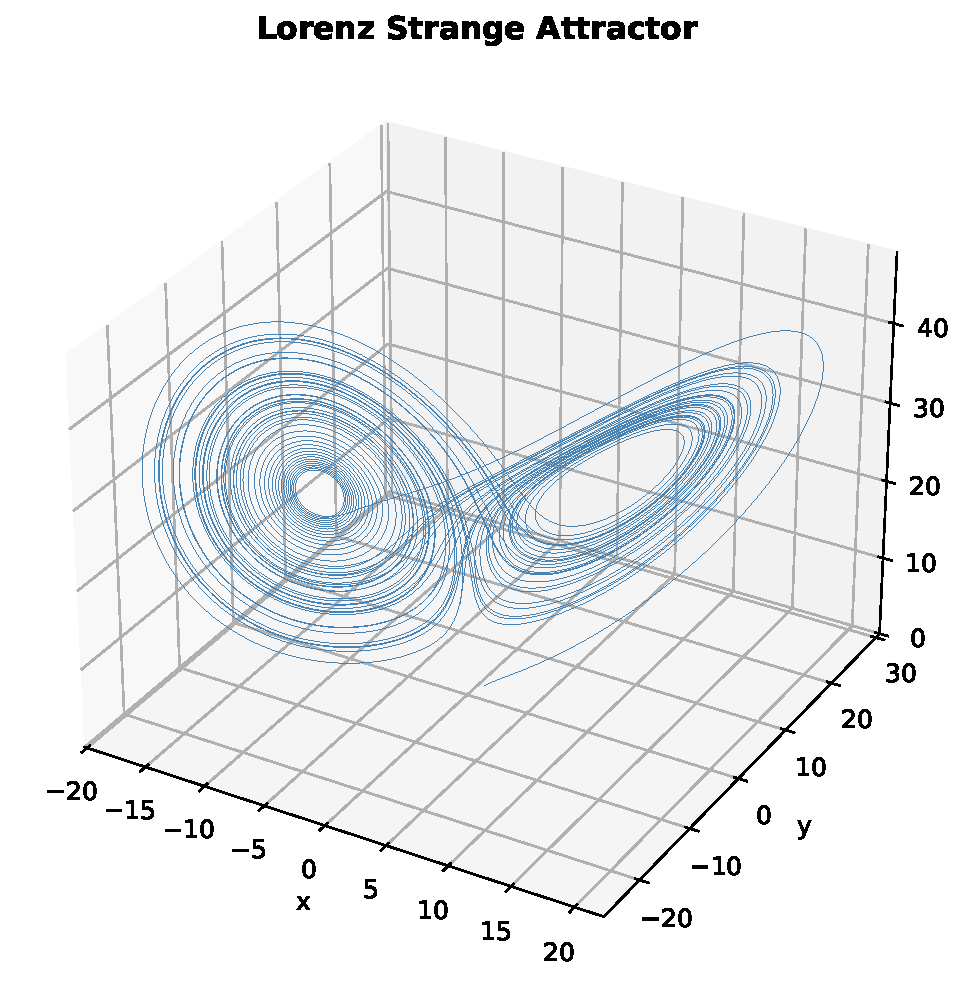
\includegraphics[width=\textwidth]{images/lorenz_attractor_3d.pdf}
    \end{center}
    \column{0.45\textwidth}
    \begin{itemize}
      \item The attractor has a butterfly-like shape with two ``wings''.
      \item Trajectories circle one wing, then unpredictably switch to the other.
      \pause
      \item It is \textbf{strange}:
      \begin{itemize}
        \item \textbf{Fractal structure}
        \item Nearby trajectories \textbf{diverge exponentially}
        \item \textbf{Zero volume} but infinite length
      \end{itemize}
    \end{itemize}
  \end{columns}
\end{frame}

\begin{frame}{2D Projections of the Attractor}
  \begin{center}
    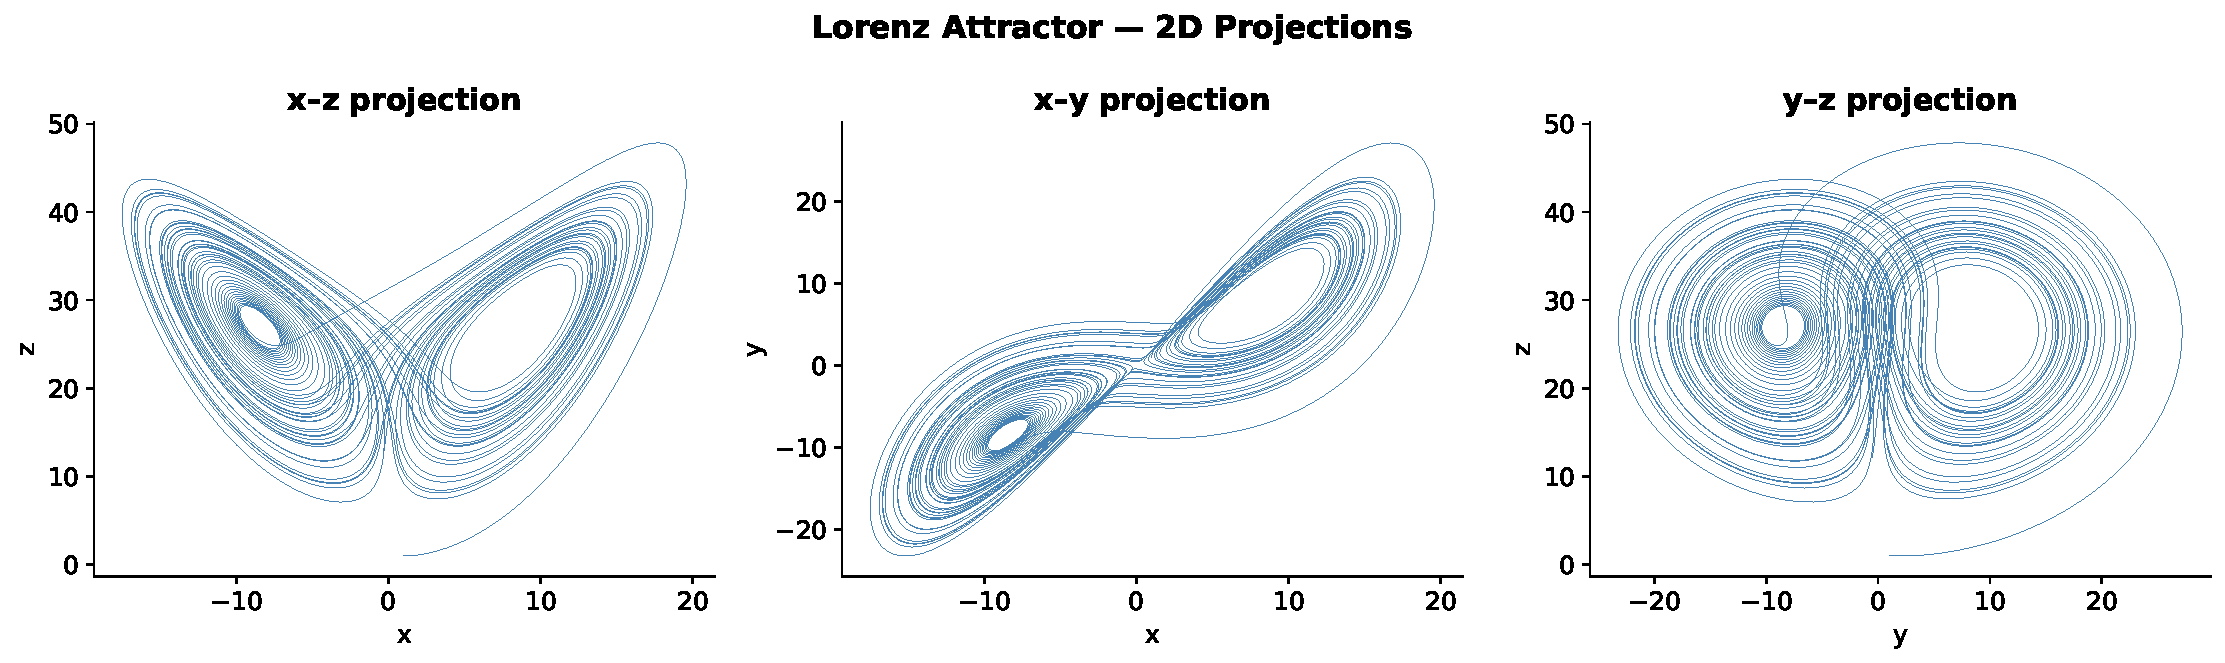
\includegraphics[width=0.95\textwidth]{images/lorenz_projections.pdf}
  \end{center}
\end{frame}

\begin{frame}{Time Series of $x(t)$}
  The $x$ component switches unpredictably between positive and negative values --- corresponding to the two wings of the attractor.
  \begin{center}
    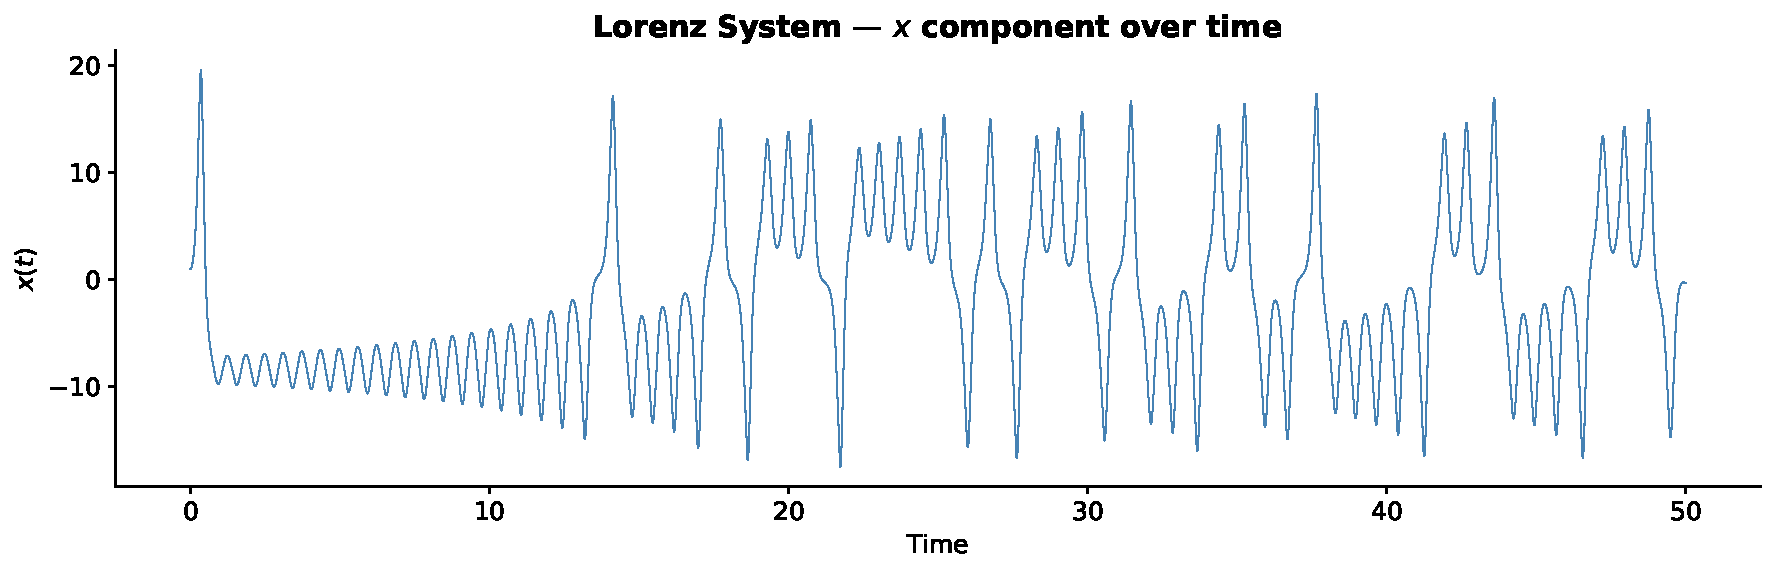
\includegraphics[width=0.9\textwidth]{images/lorenz_timeseries.pdf}
  \end{center}
\end{frame}

\begin{frame}{Sensitivity to Initial Conditions}
  \begin{itemize}
    \item Start two simulations with initial conditions differing by $10^{-9}$.
    \item For a short time, the trajectories look identical.
    \item After a critical time, they diverge completely.
  \end{itemize}
  \begin{center}
    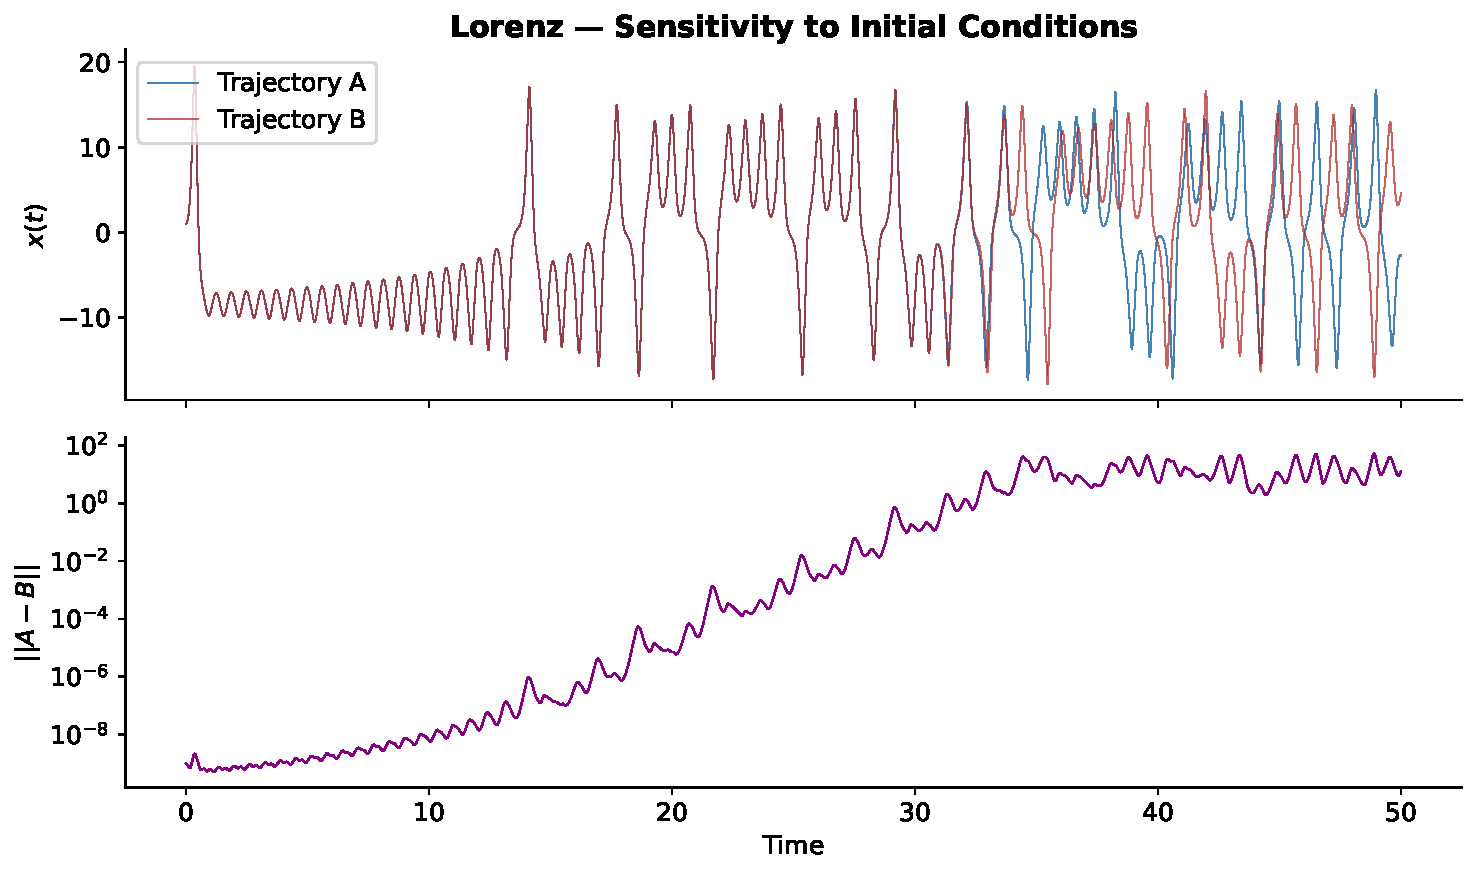
\includegraphics[width=0.82\textwidth]{images/lorenz_sensitivity.pdf}
  \end{center}
  \small
  \textbf{Deterministic but unpredictable.} The rate of divergence is measured by the \textbf{Lyapunov exponent}.
\end{frame}

\begin{frame}{Why Does This Matter?}
  \begin{itemize}
    \item The Lorenz system shows that \textbf{simple deterministic rules} can produce behaviour that \textbf{looks random}.
    \item Implications for weather forecasting:
    \begin{itemize}
      \item Accurate prediction is fundamentally limited in time.
      \item Ensemble forecasts (many slightly different initial conditions) are used to estimate uncertainty.
    \end{itemize}
    \pause
    \item The same mathematical structure appears in:
    \begin{itemize}
      \item Laser physics
      \item Chemical reactions
      \item Population dynamics
      \item Electrical circuits
      \item Climate science
    \end{itemize}
  \end{itemize}
\end{frame}
